% =============================================================================
% Mid-Review Presentation (Beamer)
% Project: Reconstruction of Tokamak Plasma State from Sparse Diagnostics
%          Using Continuous-Time Latent Dynamics Models
%
% NOTE TO TEAM: Review each narrative sentence against the cited papers before
% submission. Keep the structure, tables, equations, citations, and any
% unfilled implementation placeholders. All factual claims below were
% individually checked against the cited papers during preparation (Sept
% 2026); if you cite a specific number in your defense, re-verify it against
% the live paper, since at least one source (TokaMark) has already revised its
% numbers once.
% =============================================================================

\documentclass[aspectratio=169]{beamer}

\usetheme{Madrid}
\usecolortheme{default}
\setbeamertemplate{navigation symbols}{}
\setbeamertemplate{footline}[frame number]

\usepackage[utf8]{inputenc}
\usepackage[T1]{fontenc}
\usepackage{amsmath,amssymb}
\usepackage{graphicx}
\usepackage{booktabs}
\usepackage{array}
\usepackage{tikz}
\usetikzlibrary{arrows.meta, positioning, shapes.geometric}
\usepackage{xcolor}
\usepackage{hyperref}
\hypersetup{
  colorlinks=true, linkcolor=blue, urlcolor=blue,
  pdftitle={Robust Reconstruction of Tokamak Plasma State from Sparse Diagnostics Using Continuous-Time Neural Networks},
  pdfauthor={Kalidasan B and Nishanth D},
  pdfsubject={Mid-Review Presentation}
}

\newcolumntype{P}[1]{>{\raggedright\arraybackslash}p{#1}}

\title[Robust Plasma Reconstruction via Continuous-Time Networks]{Robust Reconstruction of Tokamak Plasma State from Sparse Diagnostics Using Continuous-Time Neural Networks}
\subtitle{Evaluating Latent Dynamics Models (CfC/LTC) Under Sensor Corruption}
\author{Kalidasan B (AM.SC.U4AIE24025) \and Nishanth D (AM.SC.U4AIE24061)}
\institute{School of Computing, Amrita Vishwa Vidyapeetham \\ Supervisor: Dr Simi S, Team Number: 14 }
\date{ 07.09.26 -- Semester 6}

\begin{document}

% ---------------------------------------------------------------------------
\begin{frame}
  \titlepage
\end{frame}

% ---------------------------------------------------------------------------
\section{Problem Statement}
\begin{frame}{Problem Statement \& Motivation}
  \textbf{Problem.} A tokamak confines plasma with magnetic fields, but no
  sensor can directly probe the plasma itself. Its magnetic state -- the 2D
  poloidal flux map $\psi(R,Z)$, which determines plasma shape and position
  -- must therefore be reconstructed from sparse external sensors, including
  flux loops, pickup coils, and coil currents.
  \vspace{4pt}

  \textbf{Current position.} Deep learning models, including CNN, CNN+LSTM,
  and a recent transformer foundation model, already perform this task well
  \textbf{on clean sensor data}. In operation, however, magnetic diagnostics
  can degrade, drop out, or fail entirely. This is especially relevant to
  next-generation reactors, where neutron damage will degrade in-vessel
  magnetics over time.
  \vspace{4pt}

  \textbf{What remains less studied.} Sensor-corruption robustness has been
  measured rigorously for a \textbf{forecasting} task, where the model
  predicts a future scalar quantity and the failure was severe. The same
  evaluation is comparatively less studied for \textbf{reconstruction},
  which recovers the current spatial state and has a different input-output
  structure. We test this directly and ask whether a continuous-time encoder
  is more robust than the standard discrete-time baseline.
\end{frame}

% ---------------------------------------------------------------------------
\section{Background}
\begin{frame}{Background / Problem Context}
  \begin{itemize}
    \item A tokamak's magnetic field shapes the plasma into nested surfaces
      described by the \textbf{poloidal flux} $\psi(R,Z)$. This 2D scalar
      field cannot be measured directly and has traditionally been obtained
      with EFIT, an iterative physics code that uses boundary magnetic
      measurements.
    \item Real diagnostics are \textbf{heterogeneous and imperfect}: flux
      loops, pickup coils, and coil currents sample at different rates and
      may be noisy, delayed, or missing. MAST diagnostics show measurable
      missing-data rates in practice.
    \item Deep learning provides a \textbf{fast, direct} sensor-to-field map
      instead of EFIT's iterative solve, and this has already worked well on
      clean data in TokaMark and TokaMind.
    \item \textbf{Continuous-time latent dynamics} (Neural ODE, LTC, CfC)
      explicitly condition the state on elapsed time, making them suited to
      irregular timing and missing inputs. In tokamak research, they have
      been used for plasma transport dynamics but not for spatial
      reconstruction.
  \end{itemize}
\end{frame}

% ---------------------------------------------------------------------------
\section{Literature Review}
\begin{frame}{Literature Review -- Overview}
  Four threads of prior work frame this project (the full set of $\sim$15
  papers appears in the separate Literature Review Table):
  \begin{enumerate}
    \item[\textbf{A.}] Reconstruction on real tokamak data -- dataset, task, and baselines
    \item[\textbf{B.}] Robustness to missing/corrupted sensors -- documented, but only for a forecasting task
    \item[\textbf{C.}] Continuous-time models in tokamak research -- applied to dynamics, never to reconstruction
    \item[\textbf{D.}] Physics-informed / alternative reconstruction approaches
  \end{enumerate}
\end{frame}

\begin{frame}{Literature Review -- Thread A: Reconstruction on Real Tokamak Data}
  \small
  \textbf{TokaMark} (Rousseau et al., IBM Research + UKAEA, 2026) is a
  public benchmark based on 11{,}573 real MAST tokamak shots (FAIR-MAST).
  It defines standardized reconstruction tasks, including flux-map
  (Task 1-3) and plasma-boundary (Task 1-2) reconstruction from sparse
  magnetics, and reports CNN and CNN+LSTM baselines. \textbf{This is the
  dataset and baseline we intend to reproduce and beat.}

  \vspace{4pt}
  \textbf{TokaMind} (Boschi et al., 2026) is a multimodal transformer
  foundation model that outperforms TokaMark's CNN baseline. It uses
  chunk-level dropout as a regularizer for missing-diagnostic robustness,
  but reports only clean-data accuracy and does not measure degradation under
  controlled sensor corruption at test time.

  \vspace{4pt}
  Related real-device work includes a DIII-D plasma-boundary reconstruction
  study using reduced diagnostics (2026) and multimodal cross-diagnostic
  super-resolution on DIII-D (Jalalvand et al., \textit{Nat.\ Commun.},
  2025). Together, these studies show that reconstruction from sparse or
  partial sensors can work \textbf{in-distribution}, while also showing that
  degraded diagnostics remain a current research concern.
\end{frame}

\begin{frame}{Literature Review -- Thread B: Robustness -- Forecasting vs.\ Reconstruction}
  \small
  \textbf{Gupta (2026)} applies a systematic robustness benchmark to
  TokaMark. LSTM, Transformer, CNN, and XGBoost models are trained on
  clean data and then evaluated under six controlled sensor-corruption
  scenarios for \textbf{Task 4-4 -- a scalar \emph{forecasting} task} that
  predicts future plasma current. The LSTM degrades by up to
  \textbf{+212\% NRMSE}, and its disruption-alarm detection rate falls to
  \textbf{0\%} when a sensor fails near the critical event. Forward-fill
  imputation largely recovers losses from random dropout.

  \vspace{6pt}
  \textbf{Important distinction.} Forecasting predicts a future value from
  past observations, whereas reconstruction recovers the \emph{current}
  spatial state from concurrent sparse sensors. The two tasks therefore have
  different input-output structures. To our knowledge, Gupta's
  train-clean/corrupt-at-test methodology has not been applied to the
  reconstruction tasks (Task 1-2/1-3) on any architecture. That is the
  reconstruction-specific evaluation gap we address.

  \vspace{6pt}
  \textbf{FusionMAE} (Yang et al., 2025) handles missing diagnostic channels
  through masked-autoencoder pretraining on HL-3 (88 channels), achieving
  96.7\% masked-channel reconstruction accuracy. It is another data-level
  fix, evaluated on signal imputation rather than 2D spatial-field
  reconstruction quality.
\end{frame}

\begin{frame}{Literature Review -- Thread C: Continuous-Time Models in Tokamak Research}
  \small
  Continuous-time models are \textbf{not new to tokamak research}, but the
  applications identified here address different problems from ours:
  \begin{itemize}
    \item Neural ODEs have been used to model \textbf{plasma transport
      dynamics} (core/edge/SOL energy exchange) on DIII-D data and to
      forecast scalar quantities such as plasma inductance on Alcator C-Mod.
      These are 0D physics-parameter fitting and scalar forecasting tasks,
      not spatial reconstruction.
    \item A \textbf{Continuous CNN} (Arnold, Spangher \& Rea, 2023) uses
      continuous convolution kernels, a different continuous-time mechanism
      from CfC/LTC. It significantly outperformed a discrete CNN for
      disruption prediction on Alcator C-Mod (AUC 0.974 vs.\ 0.799), but the
      authors explicitly state that they have \textbf{not yet tested
      robustness} to missing or corrupted data; they identify this as an open
      problem.
  \end{itemize}
  \vspace{6pt}
  \textbf{No application of a continuous-time architecture (Neural ODE, LTC,
  or CfC) to spatial plasma-state reconstruction was found.} This is the
  precise, narrow gap addressed by this project.
\end{frame}

% ---- Compact literature table for the slide deck (full ~15-paper table is the separate deliverable) ----
\begin{frame}{Literature Review -- Comparison Table (Core Papers)}
  \scriptsize
  \setlength{\tabcolsep}{2pt}
  \renewcommand{\arraystretch}{1.15}
  \begin{tabular}{P{2.1cm}P{0.45cm}P{2.2cm}P{2.2cm}P{2.4cm}P{2.6cm}}
    \toprule
    \textbf{Paper (Year)} & & \textbf{Task} & \textbf{Data} & \textbf{Key Result} & \textbf{Limitation / Relevance} \\
    \midrule
    Rousseau et al., TokaMark (arXiv:2602.10132) & 2026 &
      Flux-map / boundary reconstruction and forecasting (14 tasks) &
      11{,}573 real MAST shots (FAIR-MAST) &
      CNN+LSTM: 0.159 NRMSE (random split) $\to$ 0.257 (temporal split), Task 1-3 &
      \textbf{Our dataset and baseline}; no corruption-robustness evaluation \\
    \addlinespace
    Boschi et al., TokaMind (arXiv:2602.15084) & 2026 &
      Multimodal foundation model, all TokaMark tasks &
      Same (FAIR-MAST) &
      Outperforms the CNN baseline on Task 1-3; trains with chunk dropout &
      No systematic test-time corruption benchmark is reported \\
    \addlinespace
    Gupta, Robustness Benchmark (arXiv:2607.11915) & 2026 &
      \textit{Forecasting} (Task 4-4, plasma current) under 6 corruption scenarios &
      Same (TokaMark) &
      LSTM: +212\% NRMSE, 0\% alarm TPR under event-proximate failure &
      \textbf{Methodology template}; never applied to reconstruction tasks \\
    \addlinespace
    Arnold, Spangher \& Rea, Continuous CNN (arXiv:2312.01286) & 2023 &
      Disruption prediction (classification) &
      Alcator C-Mod &
      Continuous CNN AUC 0.974 vs.\ discrete CNN 0.799 &
      Different continuous-time mechanism; robustness is explicitly untested \\
    \addlinespace
    Rousseau et al. \textit{(consortium)}, Fusion Equilibrium Challenge (arXiv:2609.01750) & 2026 &
      Flux map reconstruction from non-magnetic diagnostics &
      8{,}794 DIII-D + 2{,}414 MAST shots &
      SSIM 0.83 in-machine $\to$ 0.10 cross-machine &
      No temporal modeling; cross-machine rather than corruption robustness \\
    \bottomrule
  \end{tabular}
\end{frame}

% ---------------------------------------------------------------------------
\section{Research Gap}
\begin{frame}{Research Gap}
  \small
  \begin{itemize}
    \item Reconstruction from sparse magnetic sensors already performs well
      \textbf{in-distribution} in TokaMark and TokaMind. Accuracy itself is
      comparatively well studied, so it is not the open problem here.
    \item Sensor-corruption robustness has been benchmarked rigorously, but
      \textbf{only for a forecasting task} (Gupta, 2026). The same
      train-clean/corrupt-at-test methodology is \textbf{comparatively less
      studied} for reconstruction and, to our knowledge, has not yet been
      applied there.
    \item Existing responses to missing or degraded sensors are
      \textbf{data-level}, such as imputation and masked pretraining. An
      \textbf{architectural} response has received less attention by
      comparison.
    \item Continuous-time models are used in tokamak research for transport
      dynamics and disruption prediction, but their use for \textbf{spatial
      state reconstruction} remains \textbf{underexplored} in the literature
      surveyed.
  \end{itemize}
  \vspace{6pt}
  \begin{block}{Gap, stated precisely (a limited-work claim, not "first-ever")}
    \small An \textbf{underexplored evaluation}: whether discrete- and
    continuous-time reconstruction models degrade gracefully or
    catastrophically under sensor corruption, and whether continuous-time
    encoders offer a measurable robustness advantage.
  \end{block}
\end{frame}

% ---------------------------------------------------------------------------
\section{Objectives}
\begin{frame}{Project Objectives}
  \begin{enumerate}
    \item Reproduce TokaMark's CNN and CNN+LSTM baselines on Task 1-3 (flux
      map) and Task 1-2 (boundary), using their published numbers as a
      correctness check.
    \item Implement a continuous-time encoder, with CfC as the primary model
      and LTC as a contrasting variant, in place of the CNN+LSTM temporal
      backbone.
    \item Define and apply a controlled sensor-corruption protocol -- random
      dropout, single-channel failure, and temporal gap -- to the test set
      only, adapting Gupta's forecasting methodology to reconstruction.
    \item Compare CNN+LSTM with CfC/LTC under identical corruption scenarios
      using NRMSE and a robustness score.
    \item Also evaluate TokaMark's temporal train/test split to check whether
      continuous-time modeling helps with the documented distribution-shift
      weakness on these tasks.
  \end{enumerate}
\end{frame}

% ---------------------------------------------------------------------------
\section{Proposed Methodology}
\begin{frame}{Proposed Methodology -- Architecture \& Data Flow}
  \begin{center}
  \resizebox{\textwidth}{!}{%
  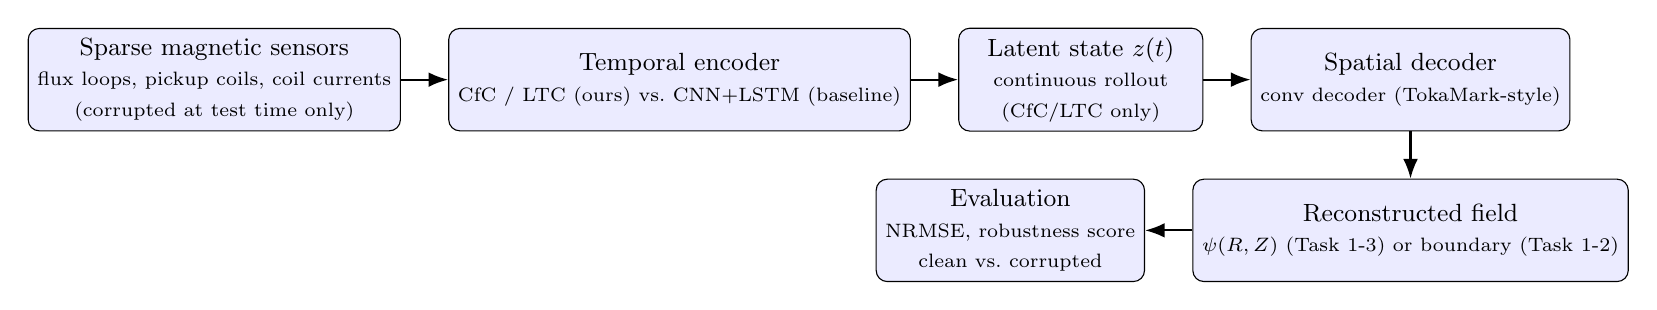
\begin{tikzpicture}[
      node distance=6mm and 6mm,
      box/.style={draw, rounded corners, minimum height=1.3cm, minimum width=3.1cm, align=center, fill=blue!8, font=\small},
      arr/.style={-{Latex[length=2.5mm]}, thick}
    ]
    \node[box] (sensors) {Sparse magnetic sensors\\ \scriptsize flux loops, pickup coils, coil currents\\ \scriptsize (corrupted at test time only)};
    \node[box, right=of sensors] (encoder) {Temporal encoder\\ \scriptsize CfC / LTC (ours) vs.\ CNN+LSTM (baseline)};
    \node[box, right=of encoder] (latent) {Latent state $z(t)$\\ \scriptsize continuous rollout\\ \scriptsize (CfC/LTC only)};
    \node[box, right=of latent] (decoder) {Spatial decoder\\ \scriptsize conv decoder (TokaMark-style)};
    \node[box, below=of decoder, minimum width=3.1cm] (output) {Reconstructed field\\ \scriptsize $\psi(R,Z)$ (Task 1-3) or boundary (Task 1-2)};
    \node[box, left=of output] (metrics) {Evaluation\\ \scriptsize NRMSE, robustness score\\ \scriptsize clean vs.\ corrupted};

    \draw[arr] (sensors) -- (encoder);
    \draw[arr] (encoder) -- (latent);
    \draw[arr] (latent) -- (decoder);
    \draw[arr] (decoder) -- (output);
    \draw[arr] (output) -- (metrics);
  \end{tikzpicture}}
  \end{center}
  \vspace{4pt}
  \small
  \textbf{Key differentiator from prior work:} the comparison changes only
  the temporal encoder. The task, data, and decoder remain the same, so the
  CNN+LSTM versus CfC/LTC comparison isolates the encoder's effect under both
  clean and corrupted conditions.
\end{frame}

\begin{frame}{Proposed Methodology -- Sensor Corruption Protocol \& Loss}
  \small
  \textbf{Corruption scenarios} are applied only to the test set, after
  training on clean data, following Gupta's train-clean/corrupt-at-test
  design:
  \begin{itemize}
    \setlength\itemsep{2pt}
    \item \textbf{Random dropout}: randomly zero a fraction (e.g.\ 10\%,
      25\%, or 50\%) of sensor readings across channels and timesteps
    \item \textbf{Single-channel failure}: remove one full sensor channel,
      such as a flux loop, for the entire input window
    \item \textbf{Temporal gap}: blank a contiguous block of timesteps to
      simulate an acquisition dropout
  \end{itemize}

  \vspace{4pt}
  \textbf{Continuous-time formulation.} The latent state evolves as a
  function of elapsed time, not step count:
  \[
    \frac{dz(t)}{dt} = f_\theta\big(z(t), x(t)\big), \qquad
    z(t) = z(t_0) + \int_{t_0}^{t} f_\theta\big(z(\tau), x(\tau)\big)\, d\tau .
  \]
  CfC solves this in closed form (without a numerical solver). A missing or
  delayed reading therefore changes the elapsed-time input rather than
  silently shifting the sequence index, as it would for an LSTM.

  \vspace{4pt}
  \textbf{Loss (reconstruction, matching TokaMark's own metric):}
  \[
    \mathcal{L}_{\text{recon}} = \text{NRMSE}\big(\hat{\psi}(R,Z),\, \psi(R,Z)\big)
  \]
\end{frame}

% ---------------------------------------------------------------------------
\section{Uniqueness}
\begin{frame}{Uniqueness / Novelty / Contribution}
  \begin{itemize}
    \item Extends Gupta's (2026) sensor-corruption benchmarking methodology
      from a \textbf{forecasting} task to a \textbf{spatial reconstruction}
      task (Task 1-2/1-3), where this evaluation approach appears
      \textbf{comparatively less studied}.
    \item Applies a continuous-time encoder, using CfC and contrasting it
      with LTC, to plasma-state reconstruction. Continuous-time models are
      established in tokamak research for transport dynamics and disruption
      prediction, but their use for spatial reconstruction has received
      \textbf{less attention} by comparison.
    \item Makes a \textbf{controlled, like-for-like architectural comparison}:
      the data and decoder stay fixed while only the temporal encoder changes.
      The comparison builds on an existing model class that has shown promise
      on tokamak time series, including Arnold et al.'s Continuous CNN, and
      examines it under a robustness lens that prior work did not apply.
    \item Frames the contribution as a \textbf{robustness evaluation and
      comparison}, not as a claim of a new state-of-the-art architecture. The
      standard CNN+LSTM baseline may already be adequately robust, which would
      be a valid and reportable outcome.
  \end{itemize}
\end{frame}

% ---------------------------------------------------------------------------
\section{Dataset \& Setup}
\begin{frame}{Dataset \& Experimental Setup}
  \small
  \textbf{Data source.} TokaMark / FAIR-MAST contains real experimental shots
  from MAST. The data are publicly streamable without credentials
  (\texttt{s3.echo.stfc.ac.uk}). We stream only the magnetics, currents, and
  flux-map signals needed for Task 1-3 (9 of 39 total signal types), rather
  than the full $\sim$2\,TB archive.

  \vspace{4pt}
  \textbf{Tasks.} The primary task is Task 1-3, flux-map reconstruction
  $\psi(R,Z)$. Task 1-2, plasma-boundary reconstruction, is a secondary and
  simpler check. TokaMark defines both tasks and provides published
  baselines.

  \vspace{4pt}
  \textbf{Baselines (published numbers to reproduce and compare against).}
  \begin{itemize}
    \setlength\itemsep{1pt}
    \item CNN: 0.148 (Task 1-3, random split) / 0.502 (temporal split)
    \item CNN+LSTM: 0.159 (Task 1-3, random split) / 0.257 (temporal split)
  \end{itemize}

  \vspace{4pt}
  \textbf{Corruption protocol.} Random dropout (10/25/50\%), single-channel
  failure, and temporal gap are applied only to the test split, following
  Gupta's clean-train / corrupt-test design (Section: Methodology).

  \vspace{2pt}
  \textbf{Environment.} PyTorch, with the \texttt{ncps} library for CfC/LTC
  cell implementations. \textit{[To be completed: specify the hardware
  (GPU/CPU) and exact package versions once finalized.]}
\end{frame}

% ---------------------------------------------------------------------------
\section{Implementation Status}
\begin{frame}{Implementation Status / Preliminary Results}
  The implementation checklist currently stands as follows:
  \vspace{4pt}
  \begin{itemize}
    \item[$\square$] TokaMark data loader set up, magnetics+currents+flux streamed
    \item[$\square$] CNN/CNN+LSTM baselines reproduced (matching published NRMSE)
    \item[$\square$] CfC/LTC encoder implemented
    \item[$\square$] Corruption protocol implemented (dropout, channel failure, temporal gap)
    \item[$\square$] Preliminary clean-vs-corrupted comparison
  \end{itemize}
  \vspace{8pt}
  \begin{center}
    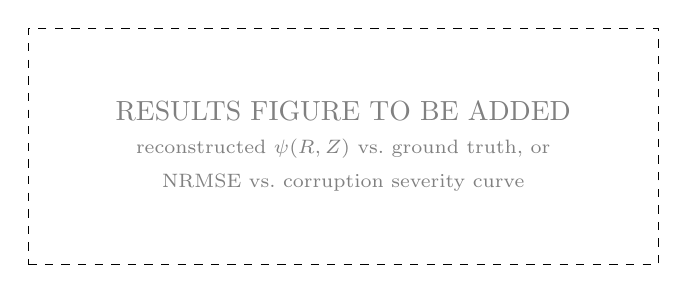
\begin{tikzpicture}
      \node[draw, dashed, minimum width=8cm, minimum height=3cm, align=center, text=gray]
        {RESULTS FIGURE TO BE ADDED\\ \scriptsize reconstructed $\psi(R,Z)$ vs.\ ground truth, or\\ \scriptsize NRMSE vs.\ corruption severity curve};
    \end{tikzpicture}
    % [FILL IN: path] -- \includegraphics[width=0.7\textwidth]{prelim_results.png}
  \end{center}
\end{frame}

% ---------------------------------------------------------------------------
\section{Challenges}
\begin{frame}{Challenges / Limitations}
  \begin{itemize}
    \item \textbf{Scope}: the project reconstructs one field, either the
      flux map or the boundary, rather than the full multi-field plasma state
      of temperature, density, and velocity. Extending it to those fields is
      future work.
    \item \textbf{Not full reactor control}: flux or boundary is only one
      input a real control system needs, alongside temperature, density, and
      disruption precursors. This project does not attempt control.
    \item \textbf{CfC implementation cost}: unlike LSTM, CfC is not a
      standard library layer, so its implementation requires care.
    \item \textbf{Baseline-number stability}: TokaMark's published numbers
      have changed between paper revisions. The reproduced baseline must be
      checked against the live version rather than assumed.
    \item \textbf{Negative-result risk}: the discrete-time baseline may
      already be adequately robust. That would be a valid, reportable outcome
      rather than a failure of the project.
  \end{itemize}
\end{frame}

% ---------------------------------------------------------------------------
\section{Work Plan}
\begin{frame}{Work Plan \& Timeline}
  \scriptsize
  \renewcommand{\arraystretch}{1.15}
  \begin{tabular}{P{6.5cm}P{2.6cm}P{2.6cm}}
    \toprule
    \textbf{Task} & \textbf{Status} & \textbf{Owner(s)} \\
    \midrule
    Literature review \& gap finalization & Completed & Kalidasan \\
    TokaMark data pipeline setup (Task 1-2/1-3) & In progress & Nishanth \\
    Reproduce CNN / CNN+LSTM baselines & In progress & Kalidasan \\
    Implement CfC / LTC encoder & Remaining & Nishanth \\
    Implement corruption protocol & Remaining & Kalidasan \\
    E1: clean-data baseline reproduction & Remaining & Nishanth \\
    E2: robustness comparison under corruption & Remaining & Nishanth \\
    E3: temporal-split generalization check & Remaining & Kalidasan \\
    Result analysis \& writeup & Remaining & Nishanth \\
    Final report \& presentation & Remaining & Kalidasan \& Nishanth \\
    \bottomrule
  \end{tabular}
  \vspace{8pt}

  \footnotesize\textit{Baseline reproduction is expected to finish within the next 1--2 days,
  leaving the remaining experiments on track for the mid-review timeline.}
\end{frame}

% ---------------------------------------------------------------------------
\section{Expected Outcomes}
\begin{frame}{Expected Outcomes \& Evaluation Plan}
  \small
  \textbf{Metrics.} NRMSE, matching TokaMark's own metric for direct
  comparability, and a robustness score based on the relative degradation
  from clean to corrupted data, following Gupta's framing.

  \vspace{4pt}
  \textbf{Experiments.}
  \begin{itemize}
    \item[E1] Reproduce the CNN/CNN+LSTM baseline on clean data as a
      correctness check
    \item[E2] Compare CNN+LSTM with CfC/LTC across dropout, channel-failure,
      and temporal-gap scenarios
    \item[E3] Evaluate the temporal split to test whether continuous-time
      modeling helps generalization as well as robustness
  \end{itemize}

  \vspace{4pt}
  \begin{block}{Anticipated outcome (a comparison, not a predetermined result)}
    On clean data, CfC/LTC is expected to be comparable to CNN+LSTM (E1).
    Under corruption (E2), the explicit elapsed-time conditioning of
    continuous-time encoders \textbf{may} support more graceful degradation
    than the discrete-time baseline. This is the hypothesis being tested, not
    an assumed conclusion. Either outcome, including a negative result with
    no meaningful difference, will be reported as a valid finding.
  \end{block}
\end{frame}

% ---------------------------------------------------------------------------
\section{References}
\begin{frame}[allowframebreaks]{References}
  \tiny
  \begin{itemize}
    \item Rousseau et al., ``TokaMark: A Comprehensive Benchmark for MAST Tokamak Plasma Models,'' arXiv:2602.10132, 2026.
    \item Boschi et al., ``TokaMind: A Multi-Modal Transformer Foundation Model for Tokamak Plasma Dynamics,'' arXiv:2602.15084, 2026.
    \item Gupta, ``Benchmarking Sensor Robustness in Plasma Diagnostic Models,'' arXiv:2607.11915, 2026.
    \item Arnold, Spangher \& Rea, ``Continuous Convolutional Neural Networks for Disruption Prediction in Nuclear Fusion Plasmas,'' arXiv:2312.01286, 2023.
    \item ``Fusion Equilibrium Challenge,'' arXiv:2609.01750 (NeurIPS-2026 benchmark), 2026.
    \item Yang et al., ``FusionMAE: pretrained model for fusion diagnostics,'' arXiv:2509.12945, 2025.
    \item Jalalvand et al., ``Multimodal Super-Resolution: Discovering Hidden Physics,'' \textit{Nat.\ Commun.}, 2025.
    \item ``Neural network reconstruction of the DIII-D tokamak plasma boundary using a reduced set of diagnostics,'' \textit{J.\ Plasma Phys.}, 2026.
    \item Joung et al., ``GS-DeepNet: mastering tokamak plasma equilibria with deep neural networks and the Grad-Shafranov equation,'' \textit{Sci.\ Rep.}, 2023.
    \item ``Application of Neural Ordinary Differential Equations for Tokamak Plasma Dynamics Analysis,'' arXiv:2403.01635, 2024.
    \item Rutigliano et al., ``Multi-diagnostics reconstruction of magnetic equilibrium and kinetic profiles using PINNs,'' \textit{Nucl.\ Fusion} 66:046006, 2026.
    \item Degrave et al., ``Magnetic control of tokamak plasmas through deep reinforcement learning,'' \textit{Nature}, 2022.
    \framebreak
    \item[] \textbf{Method background (cited in text):}
    \item Chen et al., ``Neural Ordinary Differential Equations,'' NeurIPS, 2018.
    \item Rubanova, Chen \& Duvenaud, ``Latent ODEs for Irregularly-Sampled Time Series,'' NeurIPS, 2019.
    \item Hasani et al., ``Liquid Time-constant Networks,'' AAAI, 2021.
    \item Hasani et al., ``Closed-form Continuous-time Neural Networks (CfC),'' \textit{Nat.\ Mach.\ Intell.}, 2022.
  \end{itemize}
\end{frame}

\end{document}
